% --- Template for thesis / report with tktltiki2 class ---
% 
% last updated 2013/02/15 for tkltiki2 v1.02

\documentclass[english, grading]{tktltiki2}

% tktltiki2 automatically loads babel, so you can simply
% give the language parameter (e.g. finnish, swedish, english, british) as
% a parameter for the class: \documentclass[finnish]{tktltiki2}.
% The information on title and abstract is generated automatically depending on
% the language, see below if you need to change any of these manually.
% 
% Class options:
% - grading                 -- Print labels for grading information on the front page.
% - disablelastpagecounter  -- Disables the automatic generation of page number information
%                              in the abstract. See also \numberofpagesinformation{} command below.
%
% The class also respects the following options of article class:
%   10pt, 11pt, 12pt, final, draft, oneside, twoside,
%   openright, openany, onecolumn, twocolumn, leqno, fleqn
%
% The default font size is 11pt. The paper size used is A4, other sizes are not supported.
%
% rubber: module pdftex

% --- General packages ---

\PassOptionsToPackage{hyphens}{url}
\usepackage[hyphens]{url}
\usepackage[utf8]{inputenc}
\usepackage[T1]{fontenc}
\usepackage{lmodern}
\usepackage{microtype}
\usepackage{amsfonts,amsmath,amssymb,amsthm,booktabs,color,enumitem,graphicx}
\usepackage[pdftex,hidelinks]{hyperref}
\usepackage{longtable}
\usepackage{listings}
\usepackage{diagbox}

\usepackage{algorithm}
\usepackage{algorithmic}
%\usepackage[bottom]{footmisc}

% Automatically set the PDF metadata fields
\makeatletter
\AtBeginDocument{\hypersetup{pdftitle = {\@title}, pdfauthor = {\@author}}}
\makeatother

% --- Language-related settings ---
%
% these should be modified according to your language

% babelbib for non-english bibliography using bibtex
\usepackage[fixlanguage]{babelbib}
\selectbiblanguage{english}

% add bibliography to the table of contents
\usepackage[nottoc]{tocbibind}
% tocbibind renames the bibliography, use the following to change it back
\settocbibname{References}

% -- Handy shortcuts
\newcommand{\etal}{\textit{et al}. }
\newcommand{\ie}{\textit{i}.\textit{e}., }
\newcommand{\eg}{\textit{e}.\textit{g}. }
\newcommand{\cpp}{C\texttt{++}}
\newcommand{\bolditt}[1]{\mathbf{#1}}
\newcommand{\norm}[1]{\left\lVert#1\right\rVert}

% --- Theorem environment definitions ---
\newtheorem{lau}{Lause}
\newtheorem{lem}[lau]{Lemma}
\newtheorem{kor}[lau]{Korollaari}

\theoremstyle{definition}
\newtheorem{maar}[lau]{Definition}
\newtheorem{ong}{Ongelma}
\newtheorem{alg}[lau]{Algoritmi}
\newtheorem{esim}[lau]{Esimerkki}

\theoremstyle{remark}
\newtheorem*{huom}{Huomautus}


% --- tktltiki2 options ---
%
% The following commands define the information used to generate title and
% abstract pages. The following entries should be always specified:

\title{Automatic Software Plagiarism Detection}
\author{Kristian Wahlroos}
\date{\today}
\level{M.Sc. Thesis}
\abstract{
Plagiarism is an act of copying where one doesn't rightfully credit the original source. The motivations behind plagiarism can vary from gaining economical advantage to even completing academic courses in a desperate way. Plagiarism itself exists in various domains where people want to take credit from something they have worked on. These areas can include e.g. literature, art or software.   

In this study, automatic authorship identification and plagiarism detection from software is analyzed and a model is built on top of findings. The term \textit{automatic} here refers to a system which requires as little as possible human intervention as possible. The goal for the model is to point out possible plagiarism from a collection of documents, which here is specified as a collection of source code files written by various authors. This situation closely related to authorship identification, and thus as a statistical tool, supervised machine learning model is utilized. The latter problem can be stated as \emph{given a document, which author has written this} and \emph{does this document follow the previous style of the author}. 
}

% The following can be used to specify keywords and classification of the paper:

\keywords{plagiarism; authorship identification; }

% classification according to ACM Computing Classification System (http://www.acm.org/about/class/)
% This is probably mostly relevant for computer scientists
% uncomment the following; contents of \classification will be printed under the abstract with a title
% "ACM Computing Classification System (CCS):"
% \classification{}

% If the automatic page number counting is not working as desired in your case,
% uncomment the following to manually set the number of pages displayed in the abstract page:
%
% \numberofpagesinformation{16 sivua + 10 sivua liitteissä}
%
% If you are not a computer scientist, you will want to uncomment the following by hand and specify
% your department, faculty and subject by hand:
%
% \faculty{Matemaattis-luonnontieteellinen}
% \department{Tietojenkäsittelytieteen laitos}
% \subject{Tietojenkäsittelytiede}
%
% If you are not from the University of Helsinki, then you will most likely want to set these also:
%
% \university{Helsingin Yliopisto}
% \universitylong{HELSINGIN YLIOPISTO --- HELSINGFORS UNIVERSITET --- UNIVERSITY OF HELSINKI} % displayed on the top of the abstract page
% \city{Helsinki}
%


% 10-15 pages abstract

\begin{document}

% --- Front matter ---

\frontmatter      % roman page numbering for front matter

\maketitle        % title page
\makeabstract     % abstract page

\tableofcontents  % table of contents

% --- Main matter ---

\mainmatter       % clear page, start arabic page numbering

\section{Introduction}

What means term plagiarism?
What is plagiarism?
Why studied here --> 

\section{Background}


\subsection{Source code plagiarism}
\subsubsection{Code structure}
\subsubsection{Plagiarism types}
\subsubsection{Plagiarism motives}
\subsubsection{In-class plagiarism}
\subsubsection{Plagiarism in industry}
\subsubsection{Similarity measure}
\subsection{Authorship identification}
\subsection{Machine learning}
\subsubsection{Clustering}
\subsubsection{Classification}

\newpage

\section{Related Work}
Systematic literature review was conducted as a purpose to gain an overview of the current state of source code plagiarism research. We mainly focus on methods applied in this review, to find consensus about what is held as a well-performing approach to plagiarism detection. Our review consists six key steps that follows the structure of systematic review \cite{AGCSLRIS2010}: 1) purpose, 2) details of search, 3) inclusion criteria, 4) exclusion criteria, 5) information extraction and 6) analysis. To easily conduct the review we used a web service to gather the articles.


The database that was utilized to query research papers is called \emph{Scopus\footnote{\url{https://www.scopus.com/}}}, which is a service containing peer-reviewed scientific literature. It allows users to search scientific articles by matching \eg titles, abstracts or keywords to user-defined query. The service itself maintains links to articles which are published under for example \emph{ACM (Association for Computing Machinery)} and \emph{IEEE (Institute of Electrical and Electronics Engineers)}, both of these being major computer science releases. 

Following subchapters describe how the review was conducted and what kind of results were found. We first form a categorization between studies to gain overview of the methods that are applied, then we extract statistics about data sets used in studies, and finally show the various methods that are applied to detect plagiarism. 

\subsection{Methodology}

Querying Scopus can be done in a similar way as querying databases in SQL-like languages. The query used inside Scopus as inclusion step was following
\begin{verbatim}
TITLE-ABS-KEY (("plagiarism" OR "authorship identification")  
                AND "source code") 
AND  (LIMIT-TO (SUBJAREA,"COMP"))
\end{verbatim}

\noindent
Above query translates to searching for articles which title, abstract or keywords contains the word \emph{plagiarism} or \emph{authorship identification} and the term \emph{source code}. These keywords were chosen in order to find articles which study the problem of plagiarism finding from source code either in general terms, or by utilizing authorship identification techniques. Finally, the query limits the area of study to computer science publications to find relevant methods for this thesis. 

The total number of articles gathered by querying Scopus in the inclusive search part of the literature review was 187, and the date when the query was done was 7th of February 2018. The distribution of studies per year can be seen in the following plot.

%\begin{figure}[ht]
%\centering
%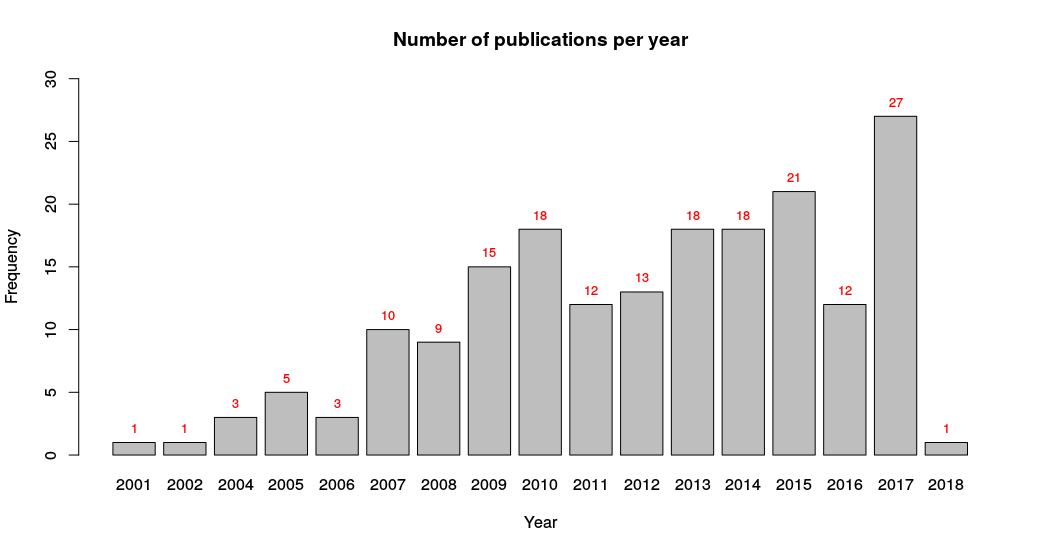
\includegraphics[width=\textwidth]{plots/Rplot.png}
%\caption{Results of inclusion phase}
%\end{figure}

\begin{figure}[ht]
\centering
\setlength\figureheight{7cm}
\setlength\figurewidth{\textwidth}
\input{plots/liter_rev/paper_distribution.tikz}
\caption{Distribution of papers per year after the inclusion phase.}
\end{figure}

After the inclusive search, we performed exclusion phase. This was done by filtering out manually all articles that were any of the following types: a review of certain aspect of source code plagiarism \eg student motives behind plagiarism, an improvement to some pre-existing algorithm \eg algorithmic speedups, plugin to online learning management systems, application to competition where the used method wasn't explained, study that used either byte-level information or information gathered during running the program, hashing techniques \eg compression and using the remaining size as a metric, system review which didn't address the method and theses. Beside these attributes, articles needed to also test their proposed method in some way and the amount of documents in experiment phase needed to be larger than two. The reason for adding this as a limiting factor was to gather studies that used test sets to evaluate the performance of their model.

The final number of articles after exclusion, and which are inspected more carefully in this systematic literature review is 32. From the set of 32 studies, we look answers for following questions: \emph{how plagiarism can be detected from source code}, \emph{what are possible features that can be derived from source code} and \emph{how can one identify the author of a given source code}. We start first by categorizing the articles by their themes to see what kind of different approaches there are to deal with the problem of plagiarism detection. After the initial classification, we summarize statistics about the data and briefly explain the used methods.


\subsection{Categorization}

The naïve categorization between articles can be done in a similar fashion as our query was constructed; dividing papers either to be about the detection of plagiarism or identifying the author of a given source code. However, as authorship identifying can also work as a way to detect plagiarism by verifying the author, we use the following high-level split visible in a table \ref{table-highcateq} where similarity detection is used as a second major category to avoid overlap.

\begin{table}[ht]
    \caption{Papers divided into two high-level categories}
    \label{table-highcateq}
    \centering
    \begin{tabular}{ | c | c | }
        
        \hline
        {\bf Similarity detection} & {\bf Authorship identification} \\ \hline
    
        \cite{AFAPLI2015, LICD2010, AASCPD2012} & \cite{SCAANN2017, ABEC2014, CAPSCAP2014}   \\
        \cite{Heblikar2015NormalizationBS, USCR2014, AIR2015} &  \cite{SCANG2007, EJPFSAI2004, ACSBPD2012}\\
        \cite{OTIOLSS2015, BUAA2009, ramirez2015high} &  \cite{APASCAI2007, UCMHGAAI2007, ESHPFSCAC2008}\\
        \cite{Ohmann2015, TBCFPD2012, Fu2017WASTKAW} &  \cite{AIRTSCAA2009, TSUDIJSCAI2011, DNNSCAI2013} \\
        \cite{ASTMLPD2013, AAPSCDPTK2013, CPDPPD2013}    & \cite{SCAIUFL2013, SDNAIJSP2015, AISC2017} \\
        \cite{PACASCD2005, RCISCP2017} &  \\ \hline
        {\bf Number of papers} & {\bf Number of papers} \\ \hline
        17 & 15 \\ \hline
    \end{tabular}
\end{table}

\noindent
Even though the articles are quite evenly divided in table \ref{table-highcateq}, these high-level groups are still too large to get a good overview of various methods. Thus we continue to categorize both groups into smaller atomic categorization, which reveals differences between and inside of them.  

Similarity detection in itself can be further divided into at least two general categories based on the current tools \cite{RSCAD2016}: attribute and structure. Then naturally, as authorship identification uses features derived directly from the source code too, we can use the same categorization to authorship identification studies. However, there are more finer categorizations that define the studies better based on the features they use, and thus we propose the following categories and their abbreviations: \emph{attribute counting (AC)}, \emph{segment matching (SM)}, \emph{n-gram (NG-STR)}, \emph{tree-based (TREE-STR)} and lastly \emph{hybrid approaches (HYB-STR)}. If a category has no studies under it, we leave the category out from the upcoming tables. These categories can be summarized briefly as following and are similar to categories identified from other plagiarism detection studies by Ali \etal \cite{OCPOCP2011}. 

\paragraph{Attribute counting}
Studies utilizing countable statistics, often referred as \emph{metrics}, that are gathered from source codes. This includes any features derived directly from source code like amount of words per line, number of lines per source code and number of keywords. For example the first two programs in appendix \ref{appendix:programs} represented as metrics is seen below.

\begin{table}[ht]
    \centering
    \begin{tabular}{|c|c|c|} \hline
        \textbf{Line count} & \textbf{Empty spaces} & \textbf{Semicolon count}\\ \hline
         10 & 1 & 5 \\ \hline
         8 & 1 & 3\\ \hline
    \end{tabular}
    \caption{First two programs in Appendix \ref{appendix:programs}; A and B represented as software metrics.}
    \label{tab:my_label}
\end{table}

\paragraph{Segment matching}
Considers two source codes as two strings and counts maximum match between them i.e. the longest common subsequence. These problems are also known as string matching problems, where one of the most famous algorithms is \emph{Greedy String Tiling} introduced early in \cite{SSGST1993}. As an example, statements \texttt{int a = 2;} and \texttt{int b = 2;} share 75\% of the character sequences and these matching sequences are: "\texttt{int}" and "\texttt{= 2;}". We also count all string similarity measures like string edit distances  to this category.

\paragraph{$N$-gram}
Treating the source code as a string and splitting it using a sliding window where the window size is the value of $n$ and the window traverses on either word or character level. This forms the vocabulary of the source code which is then transformed into occurrences of particular terms that are present, thus ultimately creating a vector representation of the source code. For example the statement \texttt{int a = 2} could be transformed into following word level 2-tuples using two as the value of $n$ (bigram). The first value of the following tuples is the $n$-gram extracted and the second value is the frequency: (\texttt{int a}, 1), (\texttt{a =}, 1), (\texttt{= 2}, 1). 

\paragraph{Tree-based}
Constructing a tree presentation from the source code, that captures the structure. For example diagram \ref{diag-parse} captures the structure of a simple assignment in parse tree, and one could compare \eg nodes of trees to define a similarity. The generation of a tree presentation usually requires some kind of parser being a very language specific feature. The inspection of a generated tree can be done with tree traversal methods for example using recursive functions. 

\paragraph{Hybrid}
Combines the usage of tree structure with $n$-gram representation. For example it can be a method which traverses abstract syntax tree, prints it and generates $n$-gram representation from the output.
\\\\
Now we can make a subcategorization for previously mentioned high-level classes; similarity detection and for authorship identification. Results for similarity detection studies can be seen from the following table, where most of them use structural features, indicated by the STR-ending. Many articles also tends to use $n$-grams to represent the source code.


\begin{table}[ht]
    \caption{Subgroups and sizes of similarity detection studies}
    \label{table-sdstudies}
    \centering
    \begin{tabular}{ | c | c | c | c | c |}
        
        \hline
        {\bf AC} & {\bf SM} & {\bf NG-STR} & {\bf AST-STR} & {\bf HYB-STR} \\ \hline
        \cite{PACASCD2005} & 
        \cite{LICD2010, ASTMLPD2013} & 
        \cite{AASCPD2012, USCR2014, AFAPLI2015} & 
        \cite{TBCFPD2012, AAPSCDPTK2013, AIR2015} & 
        \cite{BUAA2009, CPDPPD2013, RCISCP2017} \\
        & 
        & 
        \cite{Heblikar2015NormalizationBS, Ohmann2015, OTIOLSS2015} & 
        \cite{Fu2017WASTKAW} &
        \\
        & & \cite{ramirez2015high} &  & \\ \hline
        {\bf \#AC} & {\bf \#SM} & \multicolumn{3}{c |}{\bf \#STR} \\ \hline
        1 & 2 & \multicolumn{3}{c |}{14}
        \\ \hline
    \end{tabular}
\end{table}

When making the division for authorship studies, we can that in table \ref{table-aistudies} it is more evenly distributed in contrast to similarity detection articles in table \ref{table-sdstudies}. More studies now seem to utilize more countable attributes from source codes, but $n$-grams are as popular as they are in similarity detection. 

%, which is quite obvious when one considers that these methods are able to capture the writing style of an author from high-level features. For example authors can name the identifiers how they like, introduce comments and use various stylistic techniques when they write source code. 

\begin{table}[ht]
    \caption{Subgroups and sizes of authorship identification studies}
    \label{table-aistudies}
    \centering
    \begin{tabular}{ | c | c | c | c |}
        
        \hline
        {\bf AC} & {\bf NG-STR} & {\bf AST-STR} & {\bf HYB-STR} \\ \hline
        \cite{EJPFSAI2004, UCMHGAAI2007, APASCAI2007} & \cite{SCANG2007, ESHPFSCAC2008, AIRTSCAA2009} & \cite{SCAANN2017} & \cite{SDNAIJSP2015, AISC2017}\\ 
        \cite{ACSBPD2012, SCAIUFL2013, DNNSCAI2013} & \cite{TSUDIJSCAI2011, CAPSCAP2014, ABEC2014} & &\\ \hline
        {\bf \#AC} & \multicolumn{3}{c |}{\bf \#STR} \\ \hline
        6 & \multicolumn{3}{c |}{9}
        \\ \hline
    \end{tabular}
\end{table}

Results seems to show that utilizing structure is popular in both high-level classes, but quite dominant in similarity detection. Also both groups seems to show high popularity to the usage of $n$-grams, and interestingly authorship identification prefers to represent documents as statistical metrics.


\subsubsection{Data}
The data used in testing phase of 34 gathered studies is presented next, where the focus is for the similarity detection on following attributes: number of total documents, is there any synthetic data used and the average number of lines of code (Avg. LOC). For the authorship identification we focus on features like documents per author and number of possible authors. The term \emph{document} here refers to the number of source code file samples per author. We summarize the findings from data utilizing the categorization that was made earlier.

\paragraph{Similarity Detection}\mbox{}\\
Attribute counting study by Moussiades and Vakali in \cite{PACASCD2005} uses two real data sets written in C\texttt{++}. They contain programming assignments and a forged set of programs. The first data set contains 24 programs having an average of 247 lines of code per submission, the second set is 51 programs having an average of 178 lines per source code. The forged data set is two modified versions from one program, trying to deliberately confuse state-of-the-art detectors.

Segment matching study by Brixtel et al. used three corpora on their evaluation and are written in Haskell, Python and C \cite{LICD2010}. Haskell corpus had 13 documents averaging 400 lines per each, Python 15 documents averaging 150 lines per each and C 19 documents averaging 250 lines per source code. Study by Zhang and Liu used 12 programs written in C that all reflected different plagiarism strategies \cite{ASTMLPD2013}. 

Studies utilizing $n$-grams are summarized into following table.

\begin{table}[ht]
\centering
\caption{Data used in similarity detection studies utilizing $n$-grams}
\label{table-ng-str-data}
\begin{tabular}{|c|c|c|c|c|c|c|c|}
          \hline
          \backslashbox{\bf Feature}{\bf Paper} & \cite{AASCPD2012} & \cite{USCR2014} & \cite{AFAPLI2015} & \cite{Heblikar2015NormalizationBS} & \cite{Ohmann2015} & \cite{OTIOLSS2015} & \cite{ramirez2015high} \\ \hline
\bf Documents  &  179  & 5302   & 191  & 1356  & 2935  & 5408  & 1277   \\ \hline
\bf Synthetic &  No  & No  &  No  & No  & No  &  No & No  \\ \hline
\bf Avg. LOC & NA  & NA  & NA  & NA & NA  & 63.7  & NA  \\ \hline
\end{tabular}
\end{table}

\newpage

\noindent
It's visible from the table \ref{table-ng-str-data} that there are now a lot more documents used in experimentation and surprisingly synthetic data is not used at all. This is due to the usage of student submissions and competition data sets like \emph{Google Code Jam} submissions, which was for example utilized by Flores \etal in \cite{USCR2014}. 


\begin{table}[ht]
\centering
\caption{Data used in similarity detection studies utilizing abstract syntax tree}
\label{table-ast-str-data}
\begin{tabular}{|c|c|c|c|c|}
          \hline
          \backslashbox{\bf Feature}{\bf Paper} & \cite{TBCFPD2012} & \cite{AAPSCDPTK2013} & \cite{AIR2015} & \cite{Fu2017WASTKAW}\\ \hline
\bf Documents & 121 & 555 & NA & 22\,214  \\ \hline
\bf Synthetic & NA & No  & NA & Yes\\ \hline
\bf Avg. LOC & NA & 305.7 & NA & 20\\ \hline
\end{tabular}
\end{table}

\noindent
One can see from the table \ref{table-ast-str-data} that a study done by Fu \etal in \cite{Fu2017WASTKAW} has a large number of documents, and this due to two facts: they reported the size as pairs of documents and they used a generator to form a lot of forged documents from a small set of 10 original submissions. Ganguly and Jones in \cite{AIR2015} don't explicitly report the statistics of their data set, but refers to a competition test set called \emph{SOurce COde Re-use} (SOCO). This competition offers a set of C and Java files which contains known cases of cross-lingual plagiarism \cite{Flores:2014:DSC:2824864.2824878}. The train set size of SOCO is 338 files. 

Finally, hybrid study by Xiong \etal utilizes 40 assignments gathered from students \cite{BUAA2009}, Muddu \etal uses 5054 original files that they mutate to introduce copied code \cite{CPDPPD2013} and Ganguly \etal uses both train and test set of the SOCO competition, totaling around 12\,000 files \cite{RCISCP2017}. 


\paragraph{Authorship identification}\mbox{}\\
Usage of data in studies dealing with the problem of identifying the author and utilizing attribute counting are summarized to the following table, where we now turn the focus on the amount of candidate authors and documents per author reported in studies.

\begin{table}[ht]
\centering
\caption{Data used in authorship studies utilizing attribute counting}
\label{table-ai-ac-str-data}
\scalebox{0.9}{
    \begin{tabular}{|c|c|c|c|c|c|c|c|c|}
              \hline
              \backslashbox{\bf Feature}{\bf Paper} & \cite{EJPFSAI2004} & \cite{UCMHGAAI2007} & \cite{APASCAI2007} & (\cite{RA:AE2010}) & \cite{ACSBPD2012} & \cite{SCAIUFL2013} & \cite{DNNSCAI2013}\\ \hline
    \bf Authors  & 46 & 20 & 8 & 15 & 120 & 10 & 10 \\ \hline
    \bf Documents per author  & NA & 3 & 3 & 4 & NA & 61-377 & 61-377\\ \hline
    \bf Synthetic  & No & No & No & No & No & No & No\\ \hline
    \end{tabular}
}
\end{table}

\noindent
In table \ref{table-ai-ac-str-data}, one can see that there are two same data sets used in \cite{SCAIUFL2013, DNNSCAI2013}. This set was collected from \emph{SourceForge}\footnote{\url{https://sourceforge.net/}} projects and there are around 61 to 377 files per author. Rest of the attribute counting studies prefers to use \eg submissions gathered from students, as it's an easy way to gather tagged source code files.  

Next, data sets from the second popular method $n$-grams used in authorship identification, are summarized into following table.

\begin{table}[ht]
\centering
\caption{Data used in authorship studies utilizing $n$-grams}
\label{table-ai-ng-str-data}
    \begin{tabular}{|c|c|c|c|c|c|c|}
              \hline
              \backslashbox{\bf Feature}{\bf Paper} & \cite{SCANG2007} & \cite{ESHPFSCAC2008} & \cite{AIRTSCAA2009} & \cite{TSUDIJSCAI2011} & \cite{CAPSCAP2014} & \cite{ABEC2014}\\ \hline
    \bf Authors  & 100 & 8 & 100 & 8 & 30 & 30\\ \hline
    \bf Documents per author  & 14 & 2 & 14-26 & 2 & NA & NA\\ \hline
    \bf Synthetic  & No & No & No & No & No & No\\ \hline
    \end{tabular}
\end{table}

\noindent
There exists three different data sets used by three different authors in table \ref{table-ai-ng-str-data}: Burrows \etal in \cite{SCANG2007, AIRTSCAA2009} used data set gathered from students C programming assignments, Frantzeskou \etal in \cite{ESHPFSCAC2008, TSUDIJSCAI2011} used open-source programs written in Java and Tennyson \etal in \cite{CAPSCAP2014, ABEC2014} used programs written in \cpp and Java which mixture of were open-source, sample and textbook programs.

The only study that mainly used abstract syntax tree in their authorship study is by Alsulami \etal in \cite{SCAANN2017}. They used \emph{Google Code Jam} to gather 700 Python source code files belonging to 70 programmers averaging around 10 submissions per author. 

Finally, the data used in two hybrid studies are summarized. Wisse and Veenman used repositories from version control website called \emph{GitHub} \cite{SDNAIJSP2015}. The largest author pool they had while testing was 30. Zhang \etal had the data set also gathered from websites like \emph{GitHub} in their study \cite{AISC2017}. Their largest data set with respect to the author size, was imbalanced set of 503 programs belonging to 53 authors. 

\paragraph{Summary}\mbox{}\\
When looking the data usage of plagiarism study as a whole, one can see that almost all studies use data that is non-synthetic \ie use real-life data, that can be gathered for example from students course submissions or from competitions like SOCO. In similarity detection studies the median of the amount of source codes used is 447 and very few studies reported the average lines of code, which is a bit problematic as it can be easier to find plagiarism from a small set of program lines than from larger programs. In authorship attribution the median of possible authors in studies is 30 and the documents per author ranges from two to as high as 377.

% tarkista mediaani

\subsubsection{Methods}
In this chapter we turn the focus to the actual methods used in various studies. We use the same 
classification as a baseline for studies that was made earlier. The math used in studies is generalized to match the style of this paper, which means that a document is represented as $d$, matrices are bold and upper-cased $\bolditt{A}$, vectors are bold but lower-cased $\bolditt{a}$, tree structures $T$ and segments of source codes $S$ often implying strings. 

\paragraph{Similarity detection}\mbox{}\\
As a recap, the problem of similarity detection can be described formally as following.

\newtheorem*{smd}{Similarity detection}

\begin{smd}
Given a set of source code documents $D = \{d_1,...,d_n\}$, define similarity function $sim: d_i, d_j \rightarrow [0, 1]$ such that $sim(d_i, d_j) = sim(d_j, d_i)$ and $sim(d_i, d_i) = 1$, with a optional threshold $\theta \in [0, 1]$ that defines the limit where two source codes are considered as too similar. With this definition, any pair of source code file $(d_i, d_j) \in D \times D$ can also be presented as a triplet $(d_i, d_j, s)$, where $i \neq j$ and $s$ is the similarity value between documents. 
\end{smd}

The attribute counting study by Moussiades and Vakali uses a graph clustering on top of pair-wise similarities calculated using the Jaccard coefficient \cite{PACASCD2005}. Authors use following form of Jaccard coeficcient in their study where $A$ is the indexed set of substitute keywords per source code 

\begin{equation}\label{jacc_eqn}
    sim(d_1, d_2) = \dfrac{|A(d_1) \cap A(d_2)|}{|A(d_1) \cup A(d_2)|}
\end{equation}
\noindent
% refer to plag. attack
The indexed set can be built considering language dependent keywords \eg \texttt{while, for, false and true} in \cpp, and marking their position with respect to the occurrences of same keywords previously. However, authors claim that to generalize the set more, substitution keywords should be used. This means that for example all occurrences of \texttt{for}- and \texttt{while} -loops should be counted together, which helps to protect against plagiarism attack. The graph clustering algorithm Moussiades and Vakali uses is called \emph{WMajorClust} which works by presenting all pairs of source codes as non-directed graph $G = (V, E)$ where the set of vertices $V$ represents the source codes while the set of edges $E$ are weighted by equation \ref{jacc_eqn}. We can also express the definition of $E$ by Moussiades and Vakali with following constraints

\begin{equation}\label{jacc_edges_eqn}
         E = \Big\{ \{ d_i, d_j, sim(d_i, d_j)\} \, | \, (d_i, d_j) \in D \times D \land sim(d_i, d_j) \geq \theta \Big\}
\end{equation}

\noindent
%chapter ref
In equation \ref{jacc_edges_eqn}, $\theta$ is a user-defined parameter and works as a minimum threshold value that separates non-plagiarized source codes from plagiarized ones \ie two source codes will not share an edge if their similarity is below $\theta$.

Segment matching study by Brixtel \etal presents their algorithm, which builds from three major steps \cite{LICD2010}: pre-filtering, segmentation and document distance calculation. Their pre-filtering is to normalize the source code in a way, that every keyword and parameter definitions is transformed into a single symbol. As a segmentation, authors split the source code by lines forming set of segments $S_k$ presenting the partitioned set of a single source code. Similarity calculation happens by first forming distance matrix $\bolditt{M}$ between two source codes $d_1, d_2$ and then comparing all pairs of segments $(s_i^1, s_j^2) \in S_1 \times S_2$ where $S_k = (s_1^k, ..., s_n^k)$, with \emph{Levenshtein edit distance}. Distance matrix $\bolditt{M}$ is then transformed into noise reduction matrix $\bolditt{H}$ by finding the maximal matching between segmentations. Finally, $\bolditt{H}$ is filtered into a matrix $\bolditt{P}$ by convolution and utilizing a threshold\footnote{Authors used $\theta = 0.7$}. With the matrix $\bolditt{P}$, distance between two pairs of documents can be calculated by Brixtel \etal as 

\begin{equation}
    sim(d_1, d_2) = 1 - \dfrac{1}{\min(|S_1|, |S_2|)}\sum_{i, j} 1 - \bolditt{P}_{(i, j)}
\end{equation}

\noindent
Zhang and Liu utilize AST-tree and their core method is mainly constructed from two methods \cite{ASTMLPD2013}: forming the AST-representation and similarity calculation. Their AST-representation is done by traversing the parsed AST-tree and turning it into textual format by printing the nodes, and similarity calculation is computed using \emph{Smith Waterman algorithm} that finds the optimal matching between two strings $S_1, S_2$. Zhang et Liu gives the formula for similarity calculation between two source codes as

\begin{equation}
    sim(d_1, d_2) = \dfrac{2 \cdot \text{ SLength}(d_1, d_2)}{|S_1| + |S_2|}
\end{equation}
\noindent
Where SLength is the length of maximal matching string obtained via  \emph{Smith Waterman algorithm}, and $|S_k|$ represents the character length of one segment. 


$N$-gram studies take a different approach. Cosma and Joy uses \emph{Latent Semantic Analysis} to find suspicious documents \cite{AASCPD2012}. They first preprocess the documents by removing \eg short terms and comments. Then all documents are first transformed into a term-by-file matrix $\bolditt{A}$, where each document is represented as a occurrences of each unique term, which is same as forming the unigrams of a document. Values of $\bolditt{A}$ are weighted, and then $\bolditt{A}$ is decomposed via \emph{singular value decomposition} into $\bolditt{A} = \bolditt{U}\mathbf{\Sigma}\bolditt{V}^\intercal$ where $\bolditt{U}$ represents terms by dimension, $\mathbf{\Sigma}$ singular values and $\bolditt{V}$ files by dimensions. The dimensionality reduction is performed for all these matrices by considering only the first 30 columns. Finally, the similarity between a query vector $\bolditt{q}$ representing term frequency of document $d_i$, and document $d_j$ represented as a column $\bolditt{a}_j$ of matrix $\bolditt{A}$ is calculated by \emph{cosine similarity} \cite{AASCPD2012}

\begin{equation}\label{cosine_sim_eqn}
    sim(\bolditt{q}, d_j) = \cos \Theta_j = \dfrac{\bolditt{a}_j^\intercal \bolditt{q}}{\norm{\bolditt{a}_j}_2 \norm{\bolditt{q}}_2} = \dfrac{\bolditt{a}_j \boldsymbol{\cdot} \bolditt{q}}{\sqrt{\sum \limits_{i} \bolditt{a}_{(j, i)}^2} \sqrt{\sum \limits_{i} \bolditt{q}_i^2}}
\end{equation}

\noindent
Acampora and Cosma \cite{AFAPLI2015} continues on same style as Cosma and Joy \cite{AASCPD2012}, first preprocessing the documents by lowercasing and removing comments, syntactical tokens and short terms. Then using singular value decomposition with weighting to form three matrices from the corpus of source codes. For the reduced matrix $\bolditt{V}$ however, they perform a \emph{Fuzzy C-Means} clustering algorithm, which is tuned with \emph{ANFIS} learning algorithm to optimize the hyperparameters of Fuzzy C-means \cite{AFAPLI2015}. The process returns a membership degree $\mu_{i, k}$ per document, indicating how close $i$th document is to $k$th cluster. 
\noindent
Flores \etal \cite{USCR2014} uses similar preprocessing approach to Cosma and Joy. They first process the documents by lower-casing them and removing repeated character, tabs with spaces. Then transform the documents into $3$-grams and weighting them by using a \emph{term frequency}. Finally, similarity is calculated using cosine similarity where $t$ is one of the 3-grams and $tf$ is the term frequency function \cite{USCR2014}. Formally this can be calculated in a same way as in equation \ref{cosine_sim_eqn} between two documents as

\begin{equation}
    sim(d_i, d_j) = \dfrac{\sum\limits_{t \in d_i \cap d_j} tf(t, d_i) tf(t, d_j) }
                          {\sqrt{\sum\limits_{t \in d_i} tf(t, d_i)^2 \sum\limits_{t \in d_j} tf(t, d_j)^2}}
\end{equation}

\noindent
Heblikar \etal \cite{Heblikar2015NormalizationBS} preprocesses also their documents by lower-casing, pruning repeated whitespace and removing single symbols. They then normalize the documents by considering most frequent terms, renaming similar terms under same symbols and ultimately filtering them completely out from the source codes. For detection phase, they use same approach as Flores \etal did in \cite{USCR2014} but use both 1-grams and 2-grams with \emph{term frequency - inverse document frequency} (tf-idf) weighting. Interestingly, also Ramírez-de-la-Cruz \etal in \cite{OTIOLSS2015} and Ramírez-de-la-Cruz \etal in \cite{ramirez2015high} decides to use cosine similarity and Jaccard coefficient. The only major difference being, that Ramírez-de-la-Cruz \etal uses additional structural and stylistic features, forming total combination of eight various similarity measurements \cite{OTIOLSS2015}. Where as Ramírez-de-la-Cruz \etal in \cite{ramirez2015high} uses cosine similarity with character 3-grams to calculate five different similarities: lexical, stylistic, comments, text\footnote{Referring here as any string passed in as an argument of a function} and structural. Lastly, Ohmann and Rahal proposes density-based clustering to form clusters of similar documents \cite{Ohmann2015}. Their similarity approach follows closely to other studies presented above: filtering and normalization as preprocessing, data format as word $n$-grams and similarity values gained by using cosine similarity. 

Tree-based studies mostly relies on calculating similarity between two tree structures $T_i, T_j$ obtained from the original documents $d_i, d_j$ by parsing them. For example Ng \etal first generate parse tree $T$ from the source code, then decompose the parse tree into subtrees $T' \subseteq T$ with respect to the functionality \eg imports are categorized together \cite{TBCFPD2012}. The similarity score is obtained by comparing trees with \emph{depth-first search} and summing the scores for all subtrees to form a score between documents. This similarity function between two documents can be expressed with the following definition where $simST$ is the similarity score between two subtrees obtained by comparing their nodes and tokens

\begin{equation}
    sim(d_i, d_j) = sim(T_i, T_j) = \dfrac{\sum\limits_{i, j}simST(T'_i, T'_j)}{10 \cdot |T'|} \cdot 100
\end{equation}

\noindent
Son \etal computes similarity value between two parse trees with a modified parse tree kernel, and argue that their kernel function is able to consider also the length of the document \cite{AAPSCDPTK2013}. They define the kernel function $k$ via recursive function $C$ where $n$ is the node of a subtree $T'$. Function $C$ finds a maximal similarity between two nodes thus authors calls it also as the \emph{maximum node value}  

\begin{equation}
    k(T_i, T_j) = \sum\limits_{n_i \in T'_i} \sum\limits_{n_j \in T'_j} C(n_i, n_j)
\end{equation}

\noindent
The actual similarity between documents can be calculated then via normalization \cite{AAPSCDPTK2013}

\begin{equation}\label{norm_kern_eqn}
    sim(d_i, d_j) = \dfrac{k(T_i, T_j)}{\sqrt{k(T_i, T_i) \cdot k(T_j, T_j)}}
\end{equation}

% C(n_i, n_j) &= \lambda \prod \limits_{k}^{nc(n_i)} \left( 1 + \max\limits_{ch \in ch_{n_j}} C(ch_k(n_i), ch)\right)

\noindent
Another study that utilizes kernel between tree structures is by Fu \etal \cite{Fu2017WASTKAW}. They first build abstract syntax tree from a source code by normalizing and weighting nodes with term frequency–inverse document frequency, then use a tree kernel to measure similarity. Their normalization happens by transforming every variable name, array size definition and indexing of an array into single unified symbol. Then, Fu \etal remove all leaf nodes with common symbols to reduce noise, for example round and curly brackets. Finally, applied kernel method measures the edit distance of the content of expression nodes and for others, it uses calculates the similarity of subtrees with respect to their structure. In simplified way, the kernel method authors use can be expressed as dot-product between the occurances of possible subtrees expressed as vector $\bolditt{h}$ \cite{Fu2017WASTKAW}

\begin{equation}
    k(T_i, T_j) = \bolditt{h}(T_i') \boldsymbol{\cdot} \bolditt{h}(T_j')
\end{equation}

\noindent
With this definition of kernel, the similarity score between two source codes is calculated by normalizing the kernel values, leading ultimately to equation \ref{norm_kern_eqn}, which is the same as cosine similarity \cite{Fu2017WASTKAW}. The last tree-based study is by Ganguly and Jones. They use information retrieval approach and treat every document as a \emph{pseudo-query} \cite{AIR2015}. Basically this means that every document is first parsed into abstract syntax tree, then nodes belonging to similar functionality are collected together and finally specific fields are gathered from this collection by ranking them. For example all class definitions are treated as one collection and from that collection, names of the classes are extracted as weighted terms for constructing the pseudo-query. Ganguly and Jones claims that their approach allows to differentiate usage of same string literals in different situations.

Hybrid study by Xiong \etal presents their system named \textit{BUAA AntiPlagiarism} which uses abstract syntax tree to generate $n$-grams \cite{BUAA2009}. They first run the code through optimizer that gets rid of unnecessary complexity, then turn the simplified code into AST-representation and prune the tree by for example removing variable names and constants. This pruned tree is lastly travelled in preorder fashion that turns the tree into string format and form $n$-grams from that representation. To calculate similarity between documents, Xiong \etal uses Jaccard coefficient, which was defined earlier in equation \ref{jacc_eqn}, but now between sets of $n$-grams. Muddu \etal continues on combining approaches and presents their system called Code Plagiarism Detection Platform (CPDP) \cite{CPDPPD2013}. CPDP detects plagiarism by first tokenizing the AST, then turning the generated token stream into $4$-grams to be used in querying the $m$ matching documents. Finding the most closest document happens by using string matching algorithm \emph{Karp-Rabin Greedy String Tiling}, with given $n$-grams from the set of $m$ matching documents. Finally, the last similarity detection study is from Ganguly \etal in \cite{RCISCP2017}. They also use information retrieval approach in similar fashion as they did in previous work \cite{AIR2015}, to tackle with the problem related to $n$-grams without AST-representation; false-positives and exhaustive pair-wise calculation. Their method consists of building again pseudo-query and ranked list of most matching documents, where pseudo-query is built from various fields gathered from AST, for example from values of strings. With $m$ most matching documents, Ganguly \etal retrieves three kinds of features from them: lexical (3-grams); structural like identifiers, function types, and data types; and 11 stylistic features like average term length.   

\paragraph{Authorship identification}\mbox{}\\
The problem of authorship identification is very different from similarity detection. Instead of trying to find a function to represent a numerical value as similarity between two source code to detect plagiarism, authorship identification aims to reveal the writer of a document. It's common in following studies that the identification happens in closed environment, implying that the author of every document is known beforehand and can only be someone from the predefined set of possible authors. This situation can be used as authenticating and methods can be evaluated as the ground truth is known.

\newtheorem*{aui}{Authorship identification}

\begin{aui}
Given a set of documents $D$, a set of authors $A$ and a function $f: D \rightarrow A$ that identifies the writer by assigning every source code document $d \in D$ to one author $a \in A$. Estimate $f$ with $\hat{f}$, a classifier that treats every document as a feature vector $\bolditt{x}$ and every known class as a vector $\bolditt{y}$. The predicted author $\hat{y}$ can be thus expressed with $\hat{f}(\bolditt{x}) = \hat{y}$.
\end{aui}

Ding's and Samadzadeh's study follows the typical method of attribute counting studies. Authors extract total of 56 metrics belonging to three classes \cite{EJPFSAI2004}: layout, style and structure. Their feature selection is done by using variance and correlation analysis, whereas classification is done with \emph{canonical discriminant analysis}. Lange and Mancoridis extract 18 mostly text-based metrics and use genetic algorithm to find out the best combination \cite{UCMHGAAI2007}. Their classification is done by constructing a histogram per feature for every developer and then calculating which of the histograms are most closest to the unknown source code. Kothari \etal uses very similar histogram-based technique but considers style metrics and character distributions, namely character level $4$-grams \cite{APASCAI2007}. To select the most matching features for a single author, Kothari \etal uses information entropy which uses the distributions to make probabilistic evaluations. To classify the author, their approach is to have a database of writer profiles, extract metrics from source code and calculate the likelihood which known writer is the author. Arabyarmohamady \etal uses programming style to identify an author \cite{ACSBPD2012}. They build a profile for every author by transforming the source code into a feature vector \ie fingerprint and compare it to database of profiles to choose the most closest author profile. Plagiarism clusters are created by comparing the similarity of each feature vector with \emph{Euclidean distance}, thus allowing the detect issues with authorships and reveal plagiarism cases. Bandara and Wijayarathna has nine metrics that they use to generate tokens and token frequencies \cite{SCAIUFL2013}. For example, one of their metrics is number of characters per line (LLC) and to tokenize it, one creates token for specific length $n$ (LLC$_n$) and calculates the frequencies. This distribution of tokens is input to learning process called \emph{sparse auto-encoder} that learns to encode the features with neural network. Weights of this neural network are used as features to \emph{logistic regression} which classifies the author to document. Finally, similar study by again Bandara and Wijayarathna, uses now full neural networks for the same task \cite{DNNSCAI2013}. They use the same nine metrics with tokenization to get distributions per metric, and use them as a input to their deep neural network to learn to predict author from features.

Authorship identification with $n$-grams mostly use a baseline method called \emph{The Source Code Author Profile (SCAP)} in our review \cite{ESHPFSCAC2008, TSUDIJSCAI2011, CAPSCAP2014, ABEC2014}. The idea of SCAP is following: all known source codes from author $a$ are concated into one text file, $n$-grams are generated and only $L$ most frequent are kept per author to generate a profile $P$. To decide the author of a source code $d$, one calculates how many $n$-grams does unknown profile $P_d$ has in common with pre-existing author profile $P_a$

\begin{equation}
    \hat{y} = \argmax_{a \in A} |P_a \cap P_d|
\end{equation}

\noindent
The first study that uses its own method is by Burrows and Tahaghoghi. They approach the problem with information retrieval technique and consider author and document as queries \cite{SCANG2007}. Normalizing the documents is done by keeping only operators and keywords, while $n$-grams are used to present one document as overlapping sequences. Ranking the documents to create ranked list, happens with a proposed measure called \emph{Author1}. Author1-measure scores the similarity between documents and a query, and is defined using term frequencies for both query $q$ and document $d$

\begin{equation}
    \text{Author1}(q, d) = \sum\limits_{t \in q \cup d} \dfrac{1}{\min(|tf(t, q) - tf(t, d)|, 0.5)}
\end{equation}

\noindent
Burrow \etal continues on the topic of information retrieval in another study, where they experiment on six additional features on top of 6-grams \cite{AIRTSCAA2009}: white space, operators, literals, keywords, input/output (I/O) and function names. Rest of the $n$-gram related studies lean towards the SCAP method, mostly using it as a baseline while trying to improve it. For example Frantzeskou \etal analyzes the contribution of four different high-level features when using SCAP \cite{ESHPFSCAC2008}. These features are comments, layout features like spacing, identifier names and keywords. In another study, Frantzeskou \etal continues to use SCAP, but now studying the significance of user-defined identifiers with four categories \cite{TSUDIJSCAI2011}: identifiers using basic data types like \texttt{int} for integers, class identifiers, method identifiers and using all identifiers defined by the author. Tennyson and Mitropoulos study first the best profile length $L$ for SCAP \cite{CAPSCAP2014} and in another study, use two Bayesian methods to build an ensemble \cite{ABEC2014}. This ensemble works by using SCAP and Burrows method as a baseline to decide the author of a document. If there exists disagreement between baseline models, probability theory is used to classify the author. These two Bayesian methods are \emph{Maximum a Posteriori} and \emph{Bayes Optimal Classifier}, and both of them calculate probability that author $a$ wrote the document $d$ given previous data.



\newpage
\paragraph{Summary}
%\begin{algorithm}[ht]
%\caption{See how easy it is to provide algorithms}
%\label{myFirstAlgorithm}
%\begin{algorithmic}
%\REQUIRE $a$
%\STATE $b = 0$
%\STATE $x \leftarrow 1:10$
%\FORALL{x}
%    \STATE $b = b+a$
%\ENDFOR
%\RETURN $b$
%\end{algorithmic}
%\end{algorithm}

\subsubsection{Accuracies}
\input{liter_review/accuracies.tex}

\newpage


\section{Methodology}
\subsection{Context}
% Course in Uni helsinki etc.
\subsection{Data}
\subsubsection{Preprocessing}
\subsubsection{}
\subsection{Research question}

\section{Results}

\section{Discussion}

\section{Conclusion}


%

% --- References ---
%
% bibtex is used to generate the bibliography. The babplain style
% will generate numeric references (for example [1]) appropriate for theoretical
% computer science. If you need alphanumeric references (e.g [Tur90]), use
%
%\bibliographystyle{babalpha-lf}
%
% instead.
\newpage
\bibliographystyle{babplain-lf}
\bibliography{references-fi}


% --- Appendices ---

% uncomment the following

% \newpage
% \appendix
% 
% \section{Esimerkkiliite}

\end{document}
